\section{Background}

As stated above, updating page types of guest OS leads to a number of IOTLB misses, and this is related to the security policies that paravirtualized (PV) hypervisor enforces. In the PV setting, the hypervisor is responsible for protecting and update security-sensitive data structures so as to prevent illicit accesses from guest OSes and I/O devices. As Xen is typical and widely used today, this section mainly illustrates how Xen hypervisor~\cite{XEN-SOPS03} uses a x86 PV MMU model~\cite{x86-pv-model} to restrict OS-access while configures Intel IOMMU to restrict DMA-access, after which our motivation will be pointed out.

Since the model requires a familiarity with X86 address translation and related concepts, we need to understand the translation techniques first.

\subsection{understanding of address translation}

There are two address translation stages: 1) segmentation mechanism: logical address to linear address translation, which is related to GDT/LDT, and 2) paging mechanism: linear address to physical address translation, which is related to page table. In the following, we will describe the details of each stage.

\subsubsection{logical to linear address translation}

Generally, in the X86 architecture using segmentation~\cite{x86}, an instruction operand that refers to a memory location includes a value that identifies a segment and an offset within that segment. Each segment is represented by a Segment Descriptor that describes the segment characteristics, including segment base address, limitation of segment length and other meta-data. Segment Descriptors are stored in the Global Descriptor Table (GDT) or Local Descriptor Tables (LDT). Each logical address consists of a \emph{segment} selector and \emph{offset}.

To translate a logical address into a linear address, the processor does the following (see figure \ref{fig:log2lin}):

1. Uses the the segment selector to locate the segment descriptor for the segment in the \emph{GDT/LDT} and reads it into the processor.
2. Examines the segment descriptor to check the access rights and range of the segment to ensure that the segment is accessible and that the offset is within the limits of the segment. If the offset within the segment is beyond the range specified by the \emph{limit} field of the segment, the logical to linear address translation will stop as a hardware exception raise.
3. Adds the base address of the segment from the segment descriptor to the offset to form a linear address.

\begin{figure}[ht]
\centering
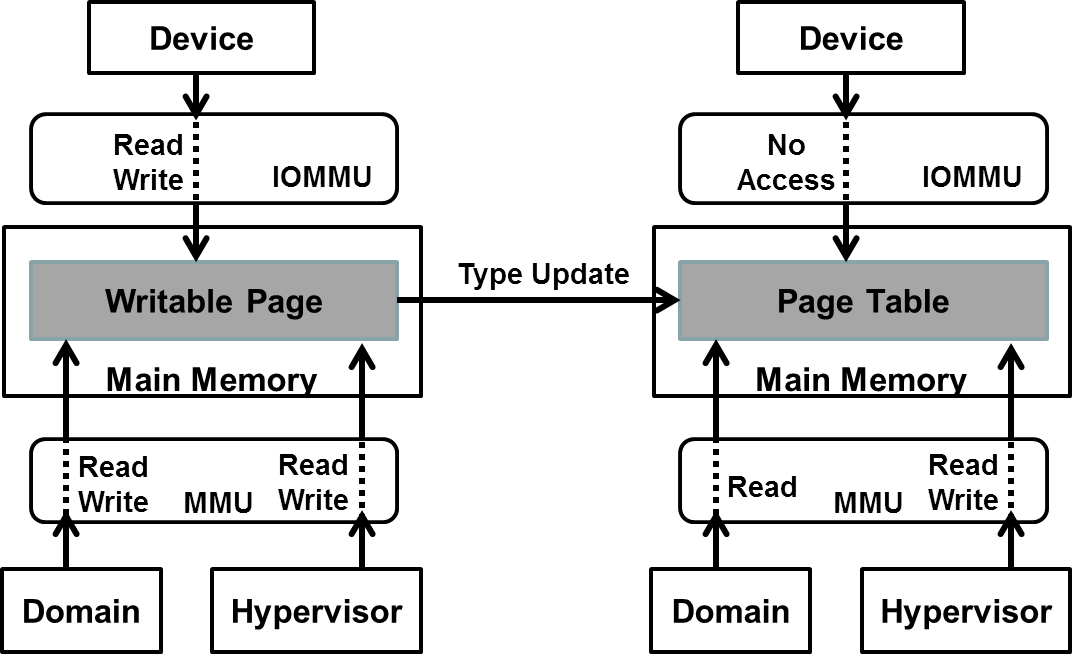
\includegraphics[width=0.5\textwidth]{image/background/log2lin.png} \\
\caption{A translation from logical address to linear address. N.B., the translation using LDT is the same process as GDT.}
\label{fig:log2lin}
\end{figure}

\subsubsection{linear to physical address translation}
To determine the physical address corresponding to a given linear address, the appropriate page table, and the correct entry within that page table must be located. Figure \ref{fig:lin2phy} illustrates the translation process when processor works in Physical Address Extension(PAE) Mode with 4K-size page~\cite{x86}.

\begin{figure}[ht]
\centering
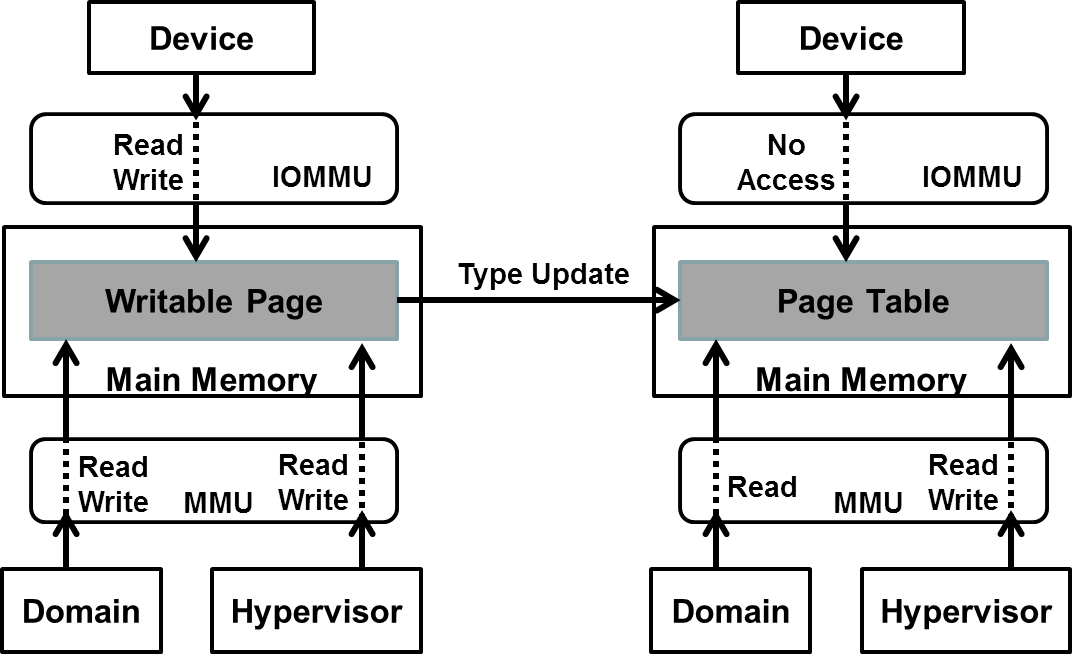
\includegraphics[width=0.5\textwidth]{image/background/lin2phy.png} \\
\caption{A translation from linear address to physical address. N.B., MMU need traverse the whole page table to find the physical address.}
\label{fig:lin2phy}
\end{figure}

Since guest kenel is working in PAE mode on the 32-bit system in the model, we use PAE-based page table to describe paging mechanism. PAE mode has 3 levels of page tables. L1 is the bottom level, L2 is the middle level and L3 is the top level. A slot in L1 is Page-Table-Entry (PTE) slot, a slot in L1 is Page-Middle-Directory (PMD) slot, and a slot in L3 is Page-Global-Directory (PGD) slot.

A given linear address is divided into 4 parts, b\_0 through b\_3. The b\_3 bits (PGD slot offset) specify an entry in the PGD page, whose base address is stored in control register CR3. The b\_1 bits (PTE slot offset) specify an entry in the PTE page, whose location is determined by the bits from b\_2 bits, which specify an entry in the PMD page respectively. Finally, processor finds the physical address by adding the offset b\_0 and the base address of the data/code page.

So far, the whole two-stage address translation is completed by hardware and thus physical memory is accessible to software. Also, to facilitate linear address translation speed, a Translation Lookaside Buffer (TLB) is used by MMU as a cache of page table entries.

\subsection{paravirtualised MMU model}

In order to prevent guest OS from subverting system, Xen PV model sets GDT/LDT and page tables be read-only. To achieve this, WP bit in the CR0 register is set, and RW bit in the PTE slots is cleared, which point to GDT/LDT and page tables. Besides, x86 architecture supports four privilege levels in hardware, ranging from ring-zero to ring-three. Typically, OS runs in ring 0, the most privileged level to execute privileged instructions, while applications executes in ring 3, the least privileged level. In the PV model, since Xen is in ring-0, it needs to modify the OS to execute in ring 1. This prevents the guest OS from executing privileged instructions to remove the read-only permissions by updating CR0.WP and RW bit in PTEs.

On top of that, Xen still applies the address translation mentioned above to the de-privileged OS. Specifically, Xen allows a direct registration of guest page tables within MMU, so that the OS has direct access to machine memory by its own page tables as well as TLB, the so called direct-paging. In the meantime, Xen must also be involved in the management of updating guest page tables to prevent OS from arbitrarily modifying its page tables, otherwise OS will have a chance to access the machine memory space of Xen since they are sharing the same virtual memory space. Also, OS cannot update the GDT/LDT as well as the Interrupt Descriptor Table (IDT) directly. Therefore, Xen limits OS to read-only access in order to protect the critical structures, provides hypercalls for OS to explicitly submit all the update requests and then validates all the requests. Note that the OS is modified to be aware that a mapping between guest physical addresses and machine addresses (P2M table) so that it can writes new page tables using machine addresses before Xen validates them.

To aid validation, Xen associates each page with a page type and a type reference count. Types are defined as following: PGT\_l1\_page\_table (used as an L1 page table), PGT\_l2\_page\_table (used as an L2 page table), PGT\_l3\_page\_table (used as an L3 page table), PGT\_l4\_page\_table (only used as an L4 page table for 64-bit x86 system), PGT\_seg\_desc\_page (used as an global descriptor table / local descriptor table), PGT\_writable\_page (a writable page). To ensure that every type is mutually exclusive and thus a given page could only have one type at every moment, the type reference count is maintained. That is to say, if the count does not drop to zero, the page type of a given page cannot be changed. With the page type and its count, Xen allows OSes to allocate and manage their own critical structures while it is only involved in updating them. Updating entries in a critical table  is a sub-operation of upating the whole table that involves a page type update. As can be seen in figure \ref{fig:page-type-update}, there are two types of updates, i.e., between writable and page-table, between writable and GDT/LDT, and we are concerned about the relationship between them and DMA-access. Note that Xen maintains the IDT directly and provides OSes with a virtual one that is not associated with any special type like GDT/LDT.

\begin{figure}[ht]
\centering
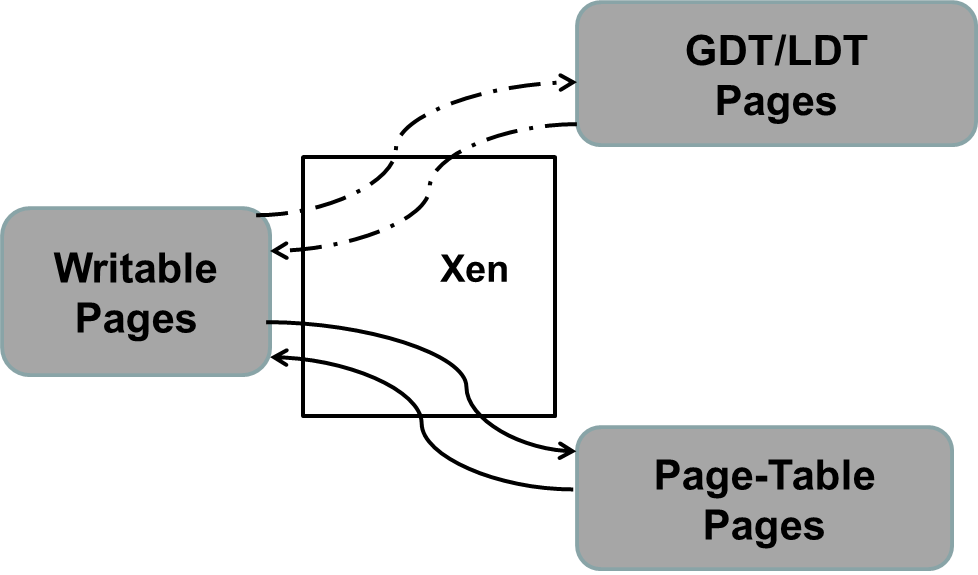
\includegraphics[width=0.5\textwidth]{image/background/page-type-update.png} \\
\caption{}
\label{fig:page-type-update}
\end{figure}

\subsection{DMA address translation}

%citing: intel vt-d
Intel IOMMU (i.e., Intel Virtualization Technology for Directed I/O)~\cite{intelvt} mainly provides hardware support for DMA Remapping and Interrupt Remapping. DMA remapping is made use of by Xen to restrict access to particular memory area from all I/O devices. DMA remapping supports independent DMA address translation, indicating that if a specific device wants to access the machine memory through DMA, the access is via I/O page tables. Xen can utilize them to do a strict examination, such as checking if the access is permitted, working like the PV MMU model. In this case, if a device is allowed to directly access specified machine memory that belongs to a guest OS, then the device is referred to as the OS's assigned devices.

More specifically, in the case of a PCI device, a DMA request is composed of two parts: a request identifier that is used to index into a specific address translation structures (i.e., multi-level page table) for a domain, and then a DMA address (also called guest physical address in Xen) is transformed by the page table to its corresponding machine address.

For a give request identifier, two tables are used to translate it into a corresponding multi-level page table, shown in figure \ref{fig: dev2dom}.

\begin{figure}[ht]
\centering
%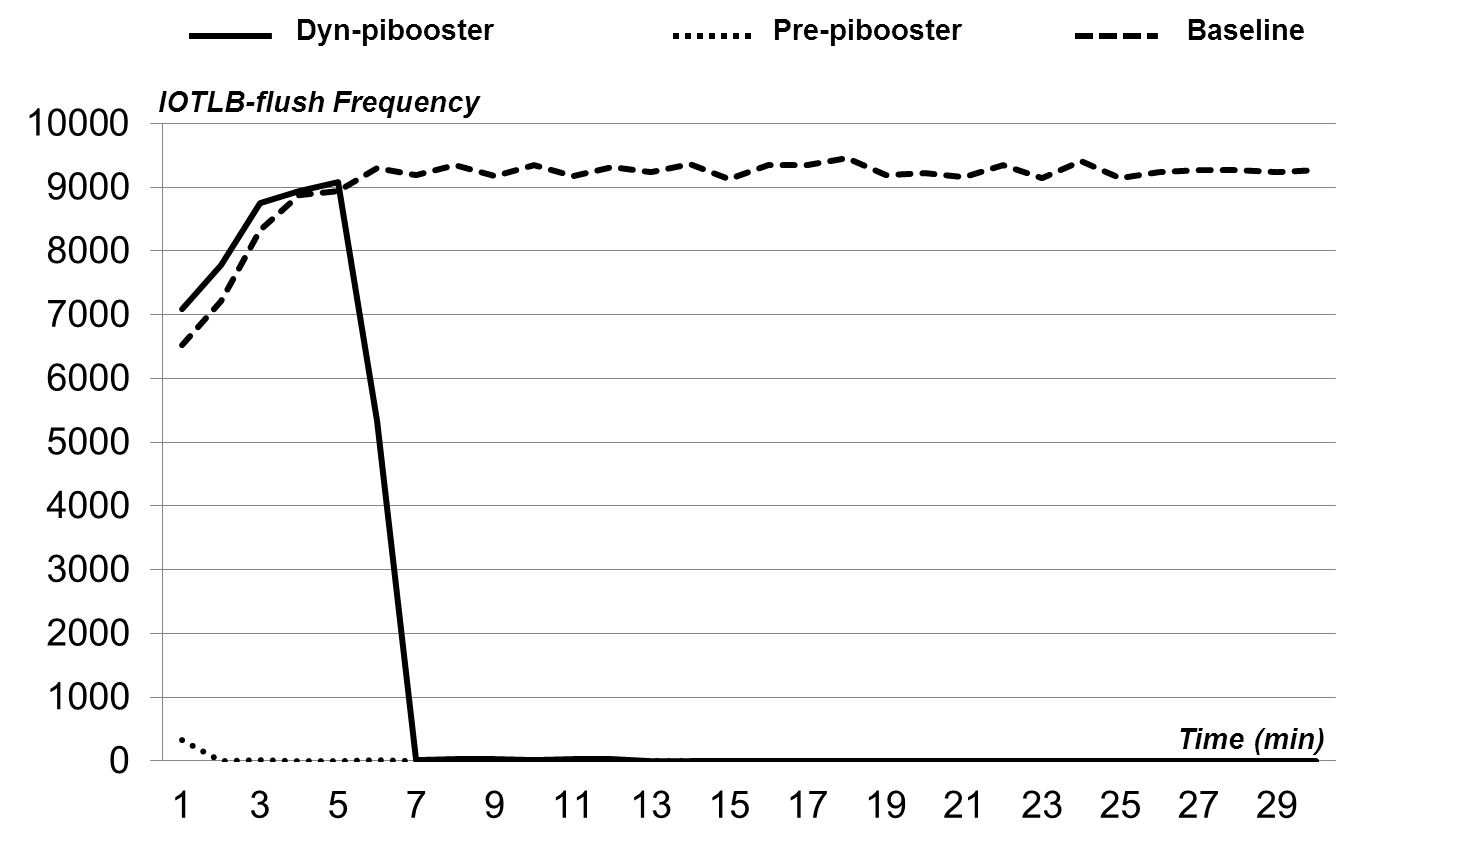
\includegraphics[scale=0.55]{image/iotlbflush.png} \\
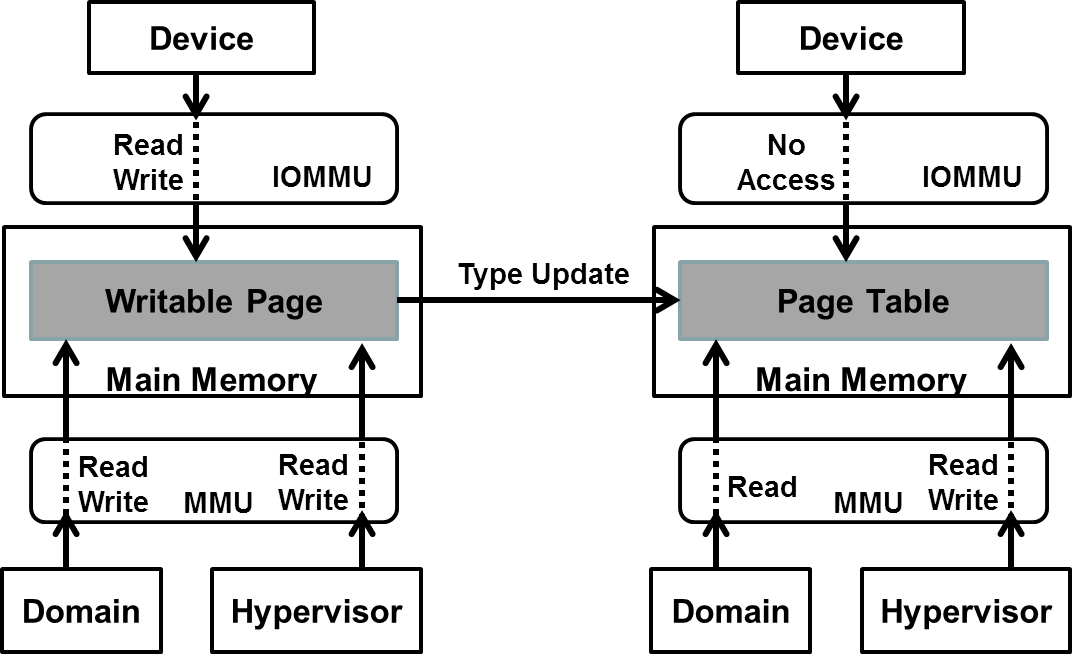
\includegraphics[width=0.5\textwidth]{image/background/dev2dom.png} \\
\caption{A mapping from the request identifier to the multi-level page table}
\label{fig: dev2dom}
\end{figure}

The request identifier has three parts. The top 8-bit representing its PCI bus number specifies an entry in the root-entry table. The device number (middle 4-bit) and function number (bottom 4-bit) are used together to index into the context-entry table, which in turn points to the base address of multi-level page table. To minimize the overhead of fetching the table entries from memory, root-entry and context-entry are cached in hardware, called the context-cache.

Multi-level, page-table-base structures translates a given DMA address to a corresponding machine address. Figure \ref{fig: gpa2ma} describes the process with a 4KB granularity of machine page, working like figure \ref{fig:lin2phy}.

\begin{figure}[ht]
\centering
%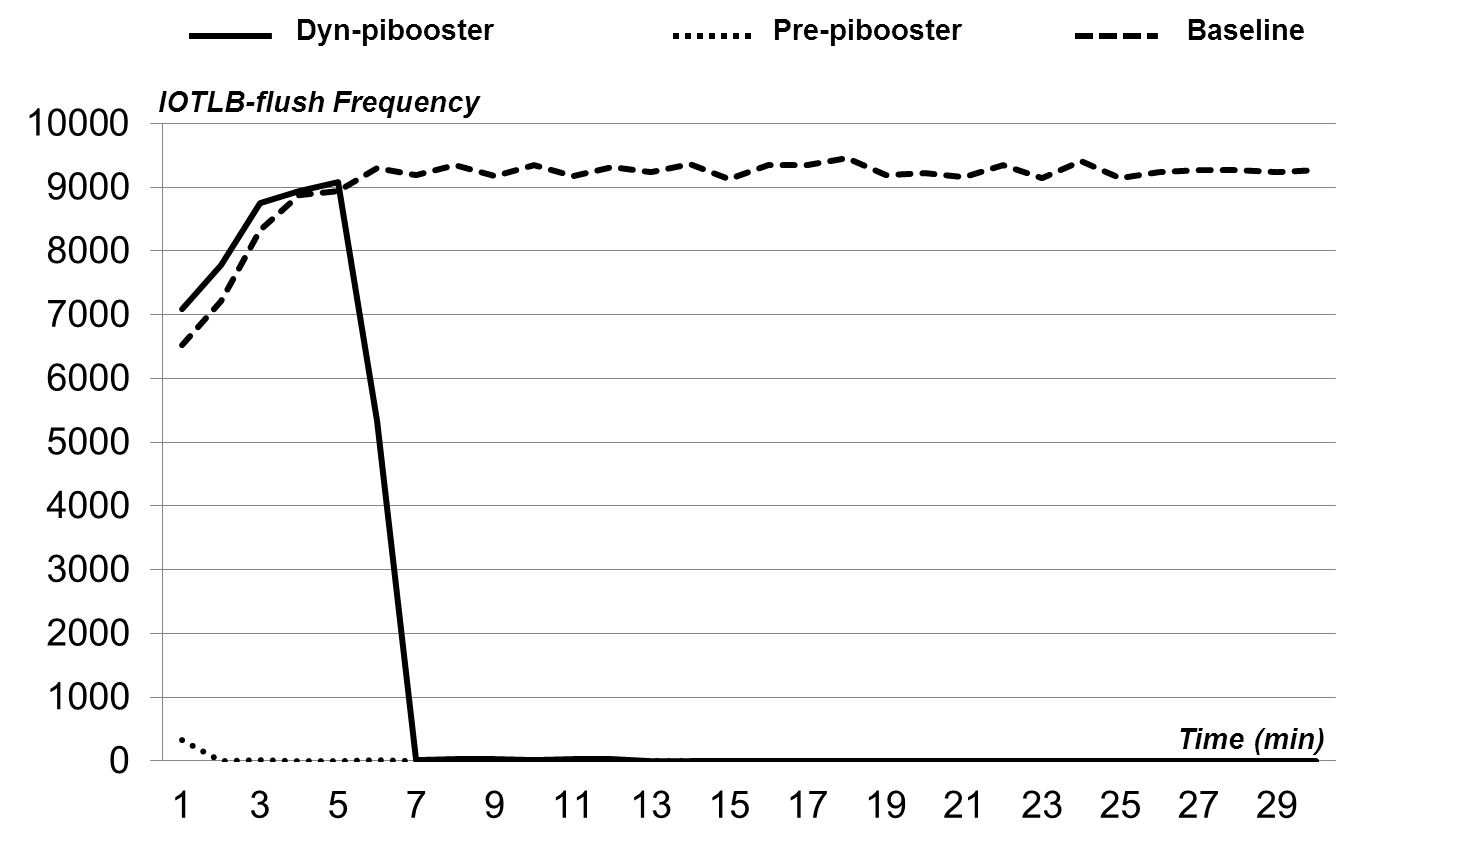
\includegraphics[scale=0.55]{image/iotlbflush.png} \\
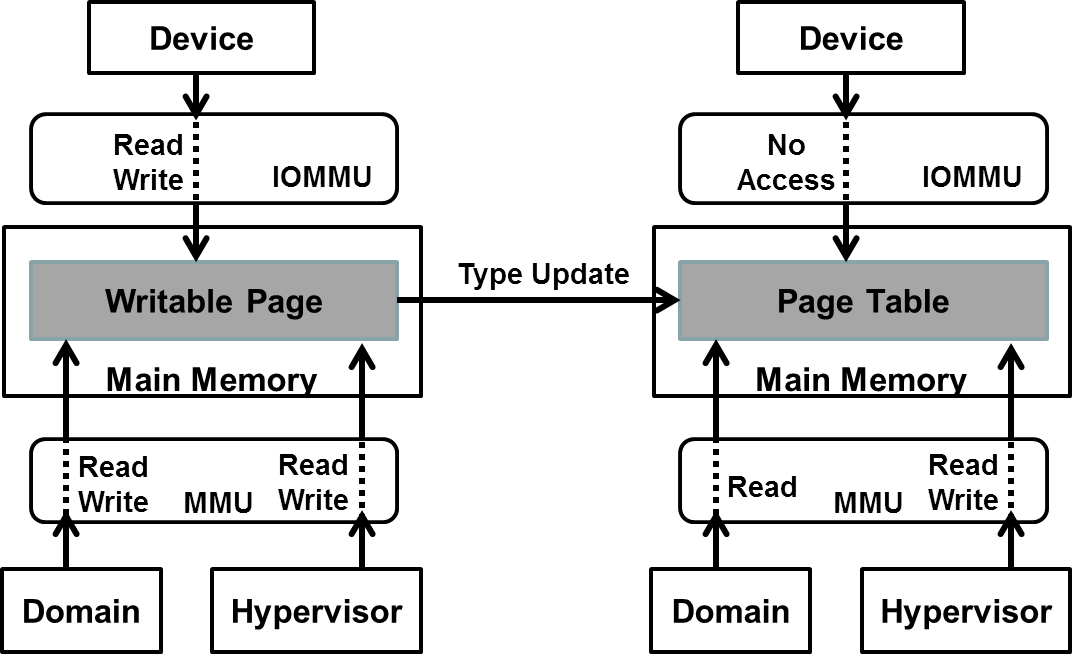
\includegraphics[width=0.5\textwidth]{image/background/gpa2ma.png} \\
\caption{A mapping from DMA address to machine address}
\label{fig: gpa2ma}
\end{figure}

Also, frequently used page tables known as the I/O translation look-aside buffer (IOTLB) are cached in hardware. Together with the context-cache, DMA remapping hardware manages them and provides cache invalidation interfaces for software. In our PV setting, Xen is responsible for explicitly invalidating corresponding caches when modifying those tables. Behaviors of invalidating IOTLB are introduced below.

%talking about how to flush IOTLB
%invalidation requests and invalidation interface

According to~\cite{intelvt}, IOMMU provides three types of IOTLB invalidation requests, i.e., global invalidation, domain-selective invalidation, page-selective invalidation. Intuitively, when requested entries in the IOTLB that correspond to specified DMA addresses need to be invalidated, a page-selective invalidation is the best choice for the sake of performance. Besides that, IOMMU also supports two kinds of invalidation interfaces: register based invalidation and queued invalidation interface, between which queued invalidation performs better.

After a brief introduction to DMA remapping, we mainly talk about how Xen utilize it to protect guest page tables from I/O devices. During the boot-up stage of a guest OS, Xen will allocate a subset of machine pages and set every writable-page in the I/O page tables as writable. Thus, both guest OS and its assigned I/O devices have write accesses to the writable pages. To prevent illicit DMA access, Xen configures the multi-level page table to make guest page-tables as well as segment descriptor tables inaccessible to devices.

As a result, when validating the page type updates from guest OS, Xen no more allows the assigned I/O device to access those to-be-page-table pages. This is where our motivation lies in.
